\documentclass[11pt,a4paper]{beamer}
\usepackage[ngerman]{babel}
\usepackage[T1]{fontenc}
\usepackage[utf8]{inputenc}
\usepackage{amsmath}
\usepackage{amsfonts}
\usepackage{amssymb}
\usepackage[normalem]{ulem}

\usepackage{tikz}
\usepackage{gantt}
\usepackage{pgf-umlcd}

\usetheme{Berlin}
\author{Julian Baumann, Xenia Kühling, Sebastian Ruder}
\title{Koreferenzresolution mit BART}
\subtitle{Abschlusssvortrag zum Softwareprojekt im Sommersemester 2014}
\date{22. Juli 2014}

\begin{document}
\maketitle

\section{Einführung}
\begin{frame}{Inhalt}
\tableofcontents
\end{frame}

\begin{frame}{Aufgabe revisited}
Grundsätzlich: System für Koreferenzresolution
\begin{itemize}
\item Vorher: BART
\item Nachher: BART mit neuem Ansatz
\begin{itemize}
\item Implementierung von vorwiegend regelbasiertem System der Stanford-NLP-Gruppe
\item Bestes Ergebnis bei CoNLL-2011 shared task
\item 10 zu implementierende Sieves, erstmal nur für Deutsch
\end{itemize}
\end{itemize}
\end{frame}


\begin{frame}{Aufbau des Stanford Systems revisited}
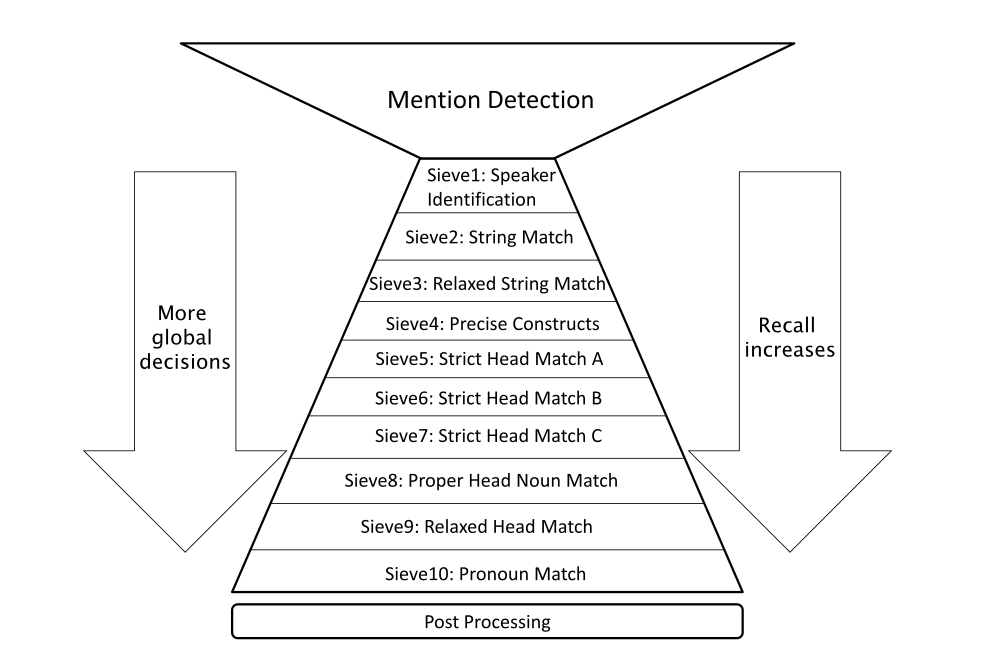
\includegraphics[scale=0.29]{stanford.png}
\end{frame}


\section{Softwarespezifikation}

\begin{frame}
\frametitle{Softwarespezifikation}

\begin{itemize}

	\item Datenformate
		\begin{itemize}
		\item MMAX2, Java, .config
	\end{itemize}
	\item BART-Version: Klon von Yannicks bitbucket \textit{repository} (\url{https://bitbucket.org/yannick/bart}); Stand 05.05.14 
	\item Korpora
	\begin{itemize}
		\item TüBA-D/Z 2008 MMAX2 (Deutsch)
		\item Penn Treebank (Englisch)
		\item Turin University Treebank/ISST (Italienisch)
	\end{itemize}
	\item Programmierumgebung
	\begin{itemize}
		\item Eclipse 4.3.2 mit IvyDE (\textit{dependency management}) sowie EGit und GitHub zur Versionskontrolle
	\end{itemize}

\end{itemize}

\end{frame}
\section{Module}

\begin{frame}
\frametitle{Endgültige Architektur}

\begin{tikzpicture}
  \begin{interface}[text width = 3cm]{corefResolver}{-1,5}  	
    \operation{decodeDocument (List<Mention> mentions, Map<Mention,Mention> antecedents : DisjointSet<Mention>)}
  \end{interface}
  
  \begin{class}[text width = 3cm]{SieveDecoder}{-1,0}    
    \implement{corefResolver}
    \attribute{sieves : List<Sieve>}
  \end{class}
  
   \begin{abstractclass}{Sieve}{5,5}
    \operation{runSieve(Mention mention, Mention potAnt) : int}
  \end{abstractclass}
  
   \begin{class}[text width = 2.5cm]{concreteSieve1}{3,0}
    \inherit{Sieve}
  \end{class}
  
   \begin{class}[text width = 2.5cm]{concreteSieve2}{7,0}
    \inherit{Sieve}
  \end{class}
  

\end{tikzpicture}
\end{frame}

\begin{frame}
\frametitle{Discourse Entity}

\begin{tikzpicture}
  \begin{class}[text width =10cm] {DiscourseEntity}{0,0}
  	\attribute{mentions : set<Mention>}
  	\attribute{\uline{nextID} : int}
  	\attribute{discourseID : ID}
    \attribute{genders : set<Gender>}
    \attribute{numbers : set<G}
	\attribute{words : set<String>}
	\attribute{heads : set<String>}
	\attribute{firstMention : Mention}
	\attribute{representativeMention : Mention}
    \operation{DiscourseEntity(Mention m)}
    
    \operation{mergeEntities(Mention m) : void}
    \operation{getMostRepresentativeMention() : void}
  \end{class}
\end{tikzpicture}

\end{frame}


\section{Demonstration!}
\begin{frame}{Demo}
Man sehe und staune! :)
\end{frame}


\section{Evaluation}
\begin{frame}{Insgesamt}
Einzufügen vorm Vortrag
\end{frame}

\begin{frame}{Vergleich mit Stanford Sieves + BART, conll 2011 shared task, Englisch}
Stanford Sieves Englisch vs. BART vs. unser BART\\

s. http://conll.cemantix.org/2011/
\end{frame}

\begin{frame}{Direkter Vergleich mit BART Deutsch}

Beispiel BART

\begin{tabular}{|c|c|c|c|}
\hline 
ID & RECALL & PRECISION & F1 \\ 
\hline 
export001 & 0.508 & 0.642 & 0.567 \\ 
\hline 
export002 & 0.467 & 0.778   & 0.584 \\ 
\hline 
export003 & 0.101 & 0.250 & 0.143 \\ 
\hline 
SCORER MUC-TOTAL & 0.457 & 0.637   & 0.532 \\
\hline

\end{tabular} 
\end{frame}

\begin{frame}{Vergleich der einzelnen Sieves}
Welches Sieve macht wie viel, eventuell Vergleich mit Stanford Sieves (welche Sieves sind bei uns toll, welche bei Stanford?)

\end{frame}
  

\section{Zeitplan}

\begin{frame}

    \begin{gantt}{10}{9}
    \begin{ganttitle}
      \titleelement{Mai}{1}
      \titleelement{Juni}{4}
      \titleelement{Juli}{4}
    \end{ganttitle}
    \begin{ganttitle}
      \titleelement{27.05.}{1}
      \titleelement{03.06.}{1}
      \titleelement{10.06.}{1}
      \titleelement{17.06.}{1}
      \titleelement{24.06.}{1}      
      \titleelement{01.07.}{1}
      \titleelement{08.07.}{1}
      \titleelement{15.07.}{1}
      \titleelement{22.07.}{1}
    \end{ganttitle}
    \ganttbar{Pipeline läuft}{0}{2}
    \ganttmilestone[color=blue]{1. \textit{Sieve} läuft}{2}
    \ganttbar{\textit{Sieves} einfügen}{2}{3}
    \ganttmilestone[color=blue]{\textit{Sieves} laufen}{5}
    \ganttbar{Evaluation}{5}{3}
    \ganttbar[color=blue]{Bugfixes}{2}{6}
    \ganttbar{Präsentation}{7}{1}
    \ganttbar[color=blue]{Dokumentation}{5}{4}
  \end{gantt}
  
\end{frame}


\section{Lessons learned, Probleme}
\begin{frame}{Probleme mit der Technik/ dem Korpus}
\begin{itemize}
\item EGit für Eclipse manchmal sehr buggy
\item Konversionsfehler im Korpus $\rightarrow$ falscher Goldstandard
\item parse- Level fehlte anfangs $\rightarrow$ Headfinder funktionierte nicht
\item TüBaD/Z Headfinder hat danach auch noch nicht richtig funktioniert $\rightarrow$ Regel in BART musste geändert werden
\end{itemize}
$\rightarrow$  FAZIT

\end{frame}


\begin{frame}{Probleme mit BART und dem Stanfordsystem}
\begin{itemize}
\item Viele Methoden in BART unklar/ nicht dokumentiert \\$\rightarrow$  Verwendung unklar
\item Modulübersicht wäre praktisch gewesen
\item Stanford Code unübersichtlich + verwirrend modularisiert\\$\rightarrow$ wenig Anreiz sich daran zu orientieren
\end{itemize}
$\rightarrow$ Immer Zeit einplanen sich in ein fremdes System einzuarbeiten!
$\rightarrow$ Sinnvollerweise jemanden haben, der kurze Einführung in System geben kann
\end{frame}



\section{Zukunft}
\begin{frame}{TO DO bis Abgabeschluss}
\begin{itemize}
\item Dokumentation beenden
\item Feinschliff an Sieves etc
\end{itemize}
\end{frame}

\begin{frame}{Weiterentwicklung}
\begin{itemize}
\item Englisch, Italienisch, andere Sprachen
\item neue Sieves 
\item verbesserte Sieves
\item BART allgemein aufräumen
\end{itemize}
\end{frame}


%\section{Quellen}
%\begin{frame}{Quellen}
%\nocite{*}
%\bibliographystyle{abbrv}
%\bibliography{lit}
%\end{frame}

\end{document}